\documentclass[twoside]{book}

% Packages required by doxygen
\usepackage{fixltx2e}
\usepackage{calc}
\usepackage{doxygen}
\usepackage[export]{adjustbox} % also loads graphicx
\usepackage{graphicx}
\usepackage[utf8]{inputenc}
\usepackage{makeidx}
\usepackage{multicol}
\usepackage{multirow}
\PassOptionsToPackage{warn}{textcomp}
\usepackage{textcomp}
\usepackage[nointegrals]{wasysym}
\usepackage[table]{xcolor}

% Font selection
\usepackage[T1]{fontenc}
\usepackage[scaled=.90]{helvet}
\usepackage{courier}
\usepackage{amssymb}
\usepackage{sectsty}
\renewcommand{\familydefault}{\sfdefault}
\allsectionsfont{%
  \fontseries{bc}\selectfont%
  \color{darkgray}%
}
\renewcommand{\DoxyLabelFont}{%
  \fontseries{bc}\selectfont%
  \color{darkgray}%
}
\newcommand{\+}{\discretionary{\mbox{\scriptsize$\hookleftarrow$}}{}{}}

% Page & text layout
\usepackage{geometry}
\geometry{%
  a4paper,%
  top=2.5cm,%
  bottom=2.5cm,%
  left=2.5cm,%
  right=2.5cm%
}
\tolerance=750
\hfuzz=15pt
\hbadness=750
\setlength{\emergencystretch}{15pt}
\setlength{\parindent}{0cm}
\setlength{\parskip}{3ex plus 2ex minus 2ex}
\makeatletter
\renewcommand{\paragraph}{%
  \@startsection{paragraph}{4}{0ex}{-1.0ex}{1.0ex}{%
    \normalfont\normalsize\bfseries\SS@parafont%
  }%
}
\renewcommand{\subparagraph}{%
  \@startsection{subparagraph}{5}{0ex}{-1.0ex}{1.0ex}{%
    \normalfont\normalsize\bfseries\SS@subparafont%
  }%
}
\makeatother

% Headers & footers
\usepackage{fancyhdr}
\pagestyle{fancyplain}
\fancyhead[LE]{\fancyplain{}{\bfseries\thepage}}
\fancyhead[CE]{\fancyplain{}{}}
\fancyhead[RE]{\fancyplain{}{\bfseries\leftmark}}
\fancyhead[LO]{\fancyplain{}{\bfseries\rightmark}}
\fancyhead[CO]{\fancyplain{}{}}
\fancyhead[RO]{\fancyplain{}{\bfseries\thepage}}
\fancyfoot[LE]{\fancyplain{}{}}
\fancyfoot[CE]{\fancyplain{}{}}
\fancyfoot[RE]{\fancyplain{}{\bfseries\scriptsize Generated by Doxygen }}
\fancyfoot[LO]{\fancyplain{}{\bfseries\scriptsize Generated by Doxygen }}
\fancyfoot[CO]{\fancyplain{}{}}
\fancyfoot[RO]{\fancyplain{}{}}
\renewcommand{\footrulewidth}{0.4pt}
\renewcommand{\chaptermark}[1]{%
  \markboth{#1}{}%
}
\renewcommand{\sectionmark}[1]{%
  \markright{\thesection\ #1}%
}

% Indices & bibliography
\usepackage{natbib}
\usepackage[titles]{tocloft}
\setcounter{tocdepth}{3}
\setcounter{secnumdepth}{5}
\makeindex

% Custom commands
\newcommand{\clearemptydoublepage}{%
  \newpage{\pagestyle{empty}\cleardoublepage}%
}

\usepackage{caption}
\captionsetup{labelsep=space,justification=centering,font={bf},singlelinecheck=off,skip=4pt,position=top}

%===== C O N T E N T S =====

\begin{document}

% Titlepage & ToC
\pagenumbering{roman}
\begin{titlepage}
\vspace*{7cm}
\begin{center}%
{\Large O\+S-\/\+Project \\[1ex]\large nachos-\/teamd }\\
\vspace*{1cm}
{\large Generated by Doxygen 1.8.11}\\
\end{center}
\end{titlepage}
\clearemptydoublepage
\tableofcontents
\clearemptydoublepage
\pagenumbering{arabic}

%--- Begin generated contents ---
\chapter{O\+S-\/\+Project -\/-\/ Team D}
\label{index}{\itshape so called \char`\"{}systemd\char`\"{} team}

This project has been realised over the the 4 project\textquotesingle{}s weeks by\+:


\begin{DoxyItemize}
\item {\tt Antoine Colombier} (Team leader)
\item {\tt Benjamin Collet}
\item {\tt Nataša Vodopivecc}
\item {\tt Philippe Ledent}
\item {\tt Sayak Samaddar}
\end{DoxyItemize}

The code documentation has been written by everyone. The main guideline and tutorial has been handled by {\tt Philippe Ledent} 
\chapter{Hierarchical Index}
\section{Class Hierarchy}
This inheritance list is sorted roughly, but not completely, alphabetically\+:\begin{DoxyCompactList}
\item \contentsline{section}{Addr\+Space}{\pageref{class_addr_space}}{}
\item \contentsline{section}{Bit\+Map}{\pageref{class_bit_map}}{}
\item \contentsline{section}{Condition}{\pageref{class_condition}}{}
\item \contentsline{section}{Console}{\pageref{class_console}}{}
\begin{DoxyCompactList}
\item \contentsline{section}{Synch\+Console}{\pageref{class_synch_console}}{}
\end{DoxyCompactList}
\item \contentsline{section}{Directory}{\pageref{class_directory}}{}
\item \contentsline{section}{Directory\+Entry}{\pageref{class_directory_entry}}{}
\item \contentsline{section}{Disk}{\pageref{class_disk}}{}
\item \contentsline{section}{File\+Header}{\pageref{class_file_header}}{}
\item \contentsline{section}{File\+System}{\pageref{class_file_system}}{}
\item \contentsline{section}{Instruction}{\pageref{class_instruction}}{}
\item \contentsline{section}{Interrupt}{\pageref{class_interrupt}}{}
\item \contentsline{section}{List}{\pageref{class_list}}{}
\item \contentsline{section}{List\+Element}{\pageref{class_list_element}}{}
\item \contentsline{section}{Lock}{\pageref{class_lock}}{}
\item \contentsline{section}{Machine}{\pageref{class_machine}}{}
\item \contentsline{section}{Mail}{\pageref{class_mail}}{}
\item \contentsline{section}{Mail\+Box}{\pageref{class_mail_box}}{}
\item \contentsline{section}{Mail\+Header}{\pageref{class_mail_header}}{}
\item \contentsline{section}{Network}{\pageref{class_network}}{}
\item \contentsline{section}{Open\+File}{\pageref{class_open_file}}{}
\item \contentsline{section}{Op\+Info}{\pageref{struct_op_info}}{}
\item \contentsline{section}{Op\+String}{\pageref{struct_op_string}}{}
\item \contentsline{section}{Packet\+Header}{\pageref{class_packet_header}}{}
\item \contentsline{section}{Pending\+Interrupt}{\pageref{class_pending_interrupt}}{}
\item \contentsline{section}{Post\+Office}{\pageref{class_post_office}}{}
\item \contentsline{section}{Scheduler}{\pageref{class_scheduler}}{}
\item \contentsline{section}{Semaphore}{\pageref{class_semaphore}}{}
\item \contentsline{section}{Statistics}{\pageref{class_statistics}}{}
\item \contentsline{section}{Synch\+Disk}{\pageref{class_synch_disk}}{}
\item \contentsline{section}{Synch\+List}{\pageref{class_synch_list}}{}
\item \contentsline{section}{Thread}{\pageref{class_thread}}{}
\item \contentsline{section}{Timer}{\pageref{class_timer}}{}
\item \contentsline{section}{Translation\+Entry}{\pageref{class_translation_entry}}{}
\end{DoxyCompactList}

\chapter{Class Index}
\section{Class List}
Here are the classes, structs, unions and interfaces with brief descriptions\+:\begin{DoxyCompactList}
\item\contentsline{section}{{\bf Addr\+Space} }{\pageref{class_addr_space}}{}
\item\contentsline{section}{{\bf Bit\+Map} }{\pageref{class_bit_map}}{}
\item\contentsline{section}{{\bf Condition} }{\pageref{class_condition}}{}
\item\contentsline{section}{{\bf Console} }{\pageref{class_console}}{}
\item\contentsline{section}{{\bf Directory} }{\pageref{class_directory}}{}
\item\contentsline{section}{{\bf Directory\+Entry} }{\pageref{class_directory_entry}}{}
\item\contentsline{section}{{\bf Disk} }{\pageref{class_disk}}{}
\item\contentsline{section}{{\bf File\+Header} }{\pageref{class_file_header}}{}
\item\contentsline{section}{{\bf File\+System} }{\pageref{class_file_system}}{}
\item\contentsline{section}{{\bf Instruction} }{\pageref{class_instruction}}{}
\item\contentsline{section}{{\bf Interrupt} }{\pageref{class_interrupt}}{}
\item\contentsline{section}{{\bf List} }{\pageref{class_list}}{}
\item\contentsline{section}{{\bf List\+Element} }{\pageref{class_list_element}}{}
\item\contentsline{section}{{\bf Lock} }{\pageref{class_lock}}{}
\item\contentsline{section}{{\bf Machine} }{\pageref{class_machine}}{}
\item\contentsline{section}{{\bf Mail} }{\pageref{class_mail}}{}
\item\contentsline{section}{{\bf Mail\+Box} }{\pageref{class_mail_box}}{}
\item\contentsline{section}{{\bf Mail\+Header} }{\pageref{class_mail_header}}{}
\item\contentsline{section}{{\bf Network} }{\pageref{class_network}}{}
\item\contentsline{section}{{\bf Open\+File} }{\pageref{class_open_file}}{}
\item\contentsline{section}{{\bf Op\+Info} }{\pageref{struct_op_info}}{}
\item\contentsline{section}{{\bf Op\+String} }{\pageref{struct_op_string}}{}
\item\contentsline{section}{{\bf Packet\+Header} }{\pageref{class_packet_header}}{}
\item\contentsline{section}{{\bf Pending\+Interrupt} }{\pageref{class_pending_interrupt}}{}
\item\contentsline{section}{{\bf Post\+Office} }{\pageref{class_post_office}}{}
\item\contentsline{section}{{\bf Scheduler} }{\pageref{class_scheduler}}{}
\item\contentsline{section}{{\bf Semaphore} }{\pageref{class_semaphore}}{}
\item\contentsline{section}{{\bf Statistics} }{\pageref{class_statistics}}{}
\item\contentsline{section}{{\bf Synch\+Console} }{\pageref{class_synch_console}}{}
\item\contentsline{section}{{\bf Synch\+Disk} }{\pageref{class_synch_disk}}{}
\item\contentsline{section}{{\bf Synch\+List} }{\pageref{class_synch_list}}{}
\item\contentsline{section}{{\bf Thread} }{\pageref{class_thread}}{}
\item\contentsline{section}{{\bf Timer} }{\pageref{class_timer}}{}
\item\contentsline{section}{{\bf Translation\+Entry} }{\pageref{class_translation_entry}}{}
\end{DoxyCompactList}

\chapter{Class Documentation}
\section{Addr\+Space Class Reference}
\label{class_addr_space}\index{Addr\+Space@{Addr\+Space}}
\subsection*{Public Member Functions}
\begin{DoxyCompactItemize}
\item 
{\bfseries Addr\+Space} ({\bf Open\+File} $\ast$executable)\label{class_addr_space_a92150df1034dc2faa393f7b9bcef8851}

\item 
void {\bfseries Init\+Registers} ()\label{class_addr_space_ab0eb6814961508ac27437b235a9296fc}

\item 
void {\bfseries Save\+State} ()\label{class_addr_space_afbdfe878dfdbc45c3fd0712ba49ebc68}

\item 
void {\bfseries Restore\+State} ()\label{class_addr_space_ac874975e4df82801d99588c35ea8252a}

\end{DoxyCompactItemize}


\subsection{Detailed Description}


Definition at line 21 of file addrspace.\+h.



The documentation for this class was generated from the following files\+:\begin{DoxyCompactItemize}
\item 
code/userprog/addrspace.\+h\item 
code/userprog/addrspace.\+cc\end{DoxyCompactItemize}

\section{Bit\+Map Class Reference}
\label{class_bit_map}\index{Bit\+Map@{Bit\+Map}}
\subsection*{Public Member Functions}
\begin{DoxyCompactItemize}
\item 
{\bfseries Bit\+Map} (int nitems)\label{class_bit_map_a957cdc72d04ce006b2efce59caa90379}

\item 
void {\bfseries Mark} (int which)\label{class_bit_map_ae3eb006c755440ae830bf220457dbbc7}

\item 
void {\bfseries Clear} (int which)\label{class_bit_map_aee4445b4d2079c96f5c87896717569d2}

\item 
bool {\bfseries Test} (int which)\label{class_bit_map_af5a945ba7b79e92a5a1bb0db24ecf26a}

\item 
int {\bfseries Find} ()\label{class_bit_map_a031ad924663dcae2359403b3a76a9dd8}

\item 
int {\bfseries Num\+Clear} ()\label{class_bit_map_af73514736aff03229d58557d0423daca}

\item 
void {\bfseries Print} ()\label{class_bit_map_a04d9c800f2a3b815f47d22c149ceae01}

\item 
void {\bfseries Fetch\+From} ({\bf Open\+File} $\ast$file)\label{class_bit_map_ad6d12eefec9b64e903d072c83f7c29a2}

\item 
void {\bfseries Write\+Back} ({\bf Open\+File} $\ast$file)\label{class_bit_map_a19052d41ba5a654c7e478582dffba20d}

\end{DoxyCompactItemize}


\subsection{Detailed Description}


Definition at line 34 of file bitmap.\+h.



The documentation for this class was generated from the following files\+:\begin{DoxyCompactItemize}
\item 
code/userprog/bitmap.\+h\item 
code/userprog/bitmap.\+cc\end{DoxyCompactItemize}

\section{Condition Class Reference}
\label{class_condition}\index{Condition@{Condition}}
\subsection*{Public Member Functions}
\begin{DoxyCompactItemize}
\item 
{\bfseries Condition} (const char $\ast$debug\+Name)\label{class_condition_a518a2676e2b33b0481f185d0f942c9c1}

\item 
const char $\ast$ {\bfseries get\+Name} () const \label{class_condition_aa7461709a0670aa96264fca1c89dda60}

\item 
void {\bfseries Wait} ({\bf Lock} $\ast$condition\+Lock)\label{class_condition_aa0442520888bd371ce07d07c0a4313a7}

\item 
void {\bfseries Signal} ({\bf Lock} $\ast$condition\+Lock)\label{class_condition_ada25a70d161b7dc9b81eaad0ef66d91c}

\item 
void {\bfseries Broadcast} ({\bf Lock} $\ast$condition\+Lock)\label{class_condition_aefae94b3f9be40a09df667e63a4bdab7}

\end{DoxyCompactItemize}


\subsection{Detailed Description}


Definition at line 131 of file synch.\+h.



The documentation for this class was generated from the following files\+:\begin{DoxyCompactItemize}
\item 
code/threads/synch.\+h\item 
code/threads/synch.\+cc\end{DoxyCompactItemize}

\section{Console Class Reference}
\label{class_console}\index{Console@{Console}}


Inheritance diagram for Console\+:\nopagebreak
\begin{figure}[H]
\begin{center}
\leavevmode
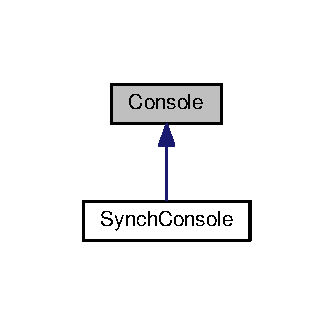
\includegraphics[width=160pt]{class_console__inherit__graph}
\end{center}
\end{figure}
\subsection*{Public Member Functions}
\begin{DoxyCompactItemize}
\item 
{\bfseries Console} (char $\ast$read\+File, char $\ast$write\+File, Void\+Function\+Ptr read\+Avail, Void\+Function\+Ptr write\+Done, int call\+Arg)\label{class_console_a406c2b2b53d474272656d7ec934b7235}

\item 
virtual void {\bfseries Put\+Char} (char ch)\label{class_console_af4828702d63f7f144e8d17395471b59f}

\item 
virtual int {\bfseries Get\+Char} ()\label{class_console_a871a3f4742f6481b903a360179d8f4a7}

\item 
void {\bfseries Write\+Done} ()\label{class_console_a8a611e74235a39a9b7216b6d66e32c30}

\item 
void {\bfseries Check\+Char\+Avail} ()\label{class_console_a099797597b7bd0b349518aac215fcb2f}

\end{DoxyCompactItemize}


\subsection{Detailed Description}


Definition at line 38 of file console.\+h.



The documentation for this class was generated from the following files\+:\begin{DoxyCompactItemize}
\item 
code/machine/console.\+h\item 
code/machine/console.\+cc\end{DoxyCompactItemize}

\section{Directory Class Reference}
\label{class_directory}\index{Directory@{Directory}}
\subsection*{Public Member Functions}
\begin{DoxyCompactItemize}
\item 
{\bfseries Directory} (int size)\label{class_directory_a77366fc5c4d73a3c20fc060640b1258a}

\item 
void {\bfseries Fetch\+From} ({\bf Open\+File} $\ast$file)\label{class_directory_a36ed455b21bbd9a66ffe8ec689ff7c73}

\item 
void {\bfseries Write\+Back} ({\bf Open\+File} $\ast$file)\label{class_directory_abf5550df42587bbc604c71441a4d12fc}

\item 
int {\bfseries Find} (const char $\ast$name)\label{class_directory_abfe376d1883918703cda2a6a4e23ffa8}

\item 
bool {\bfseries Add} (const char $\ast$name, int new\+Sector)\label{class_directory_aab3700537a499e57a07c79ba666d2fcb}

\item 
bool {\bfseries Remove} (const char $\ast$name)\label{class_directory_a3ad4280cbe376ef803105e6a35856165}

\item 
void {\bfseries List} ()\label{class_directory_a5065793fb216a407cc3871dd3c837117}

\item 
void {\bfseries Print} ()\label{class_directory_a40c728221c5557e4fc181c4091c6fcff}

\end{DoxyCompactItemize}


\subsection{Detailed Description}


Definition at line 51 of file directory.\+h.



The documentation for this class was generated from the following files\+:\begin{DoxyCompactItemize}
\item 
code/filesys/directory.\+h\item 
code/filesys/directory.\+cc\end{DoxyCompactItemize}

\section{Directory\+Entry Class Reference}
\label{class_directory_entry}\index{Directory\+Entry@{Directory\+Entry}}
\subsection*{Public Attributes}
\begin{DoxyCompactItemize}
\item 
bool {\bfseries in\+Use}\label{class_directory_entry_a0686edcff271cdb66a2cb19696e7200a}

\item 
int {\bfseries sector}\label{class_directory_entry_afe912144a818d7884e3f22c842cac3c5}

\item 
char {\bfseries name} [File\+Name\+Max\+Len+1]\label{class_directory_entry_aee1f8d0797adfa14488f4e4516118664}

\end{DoxyCompactItemize}


\subsection{Detailed Description}


Definition at line 32 of file directory.\+h.



The documentation for this class was generated from the following file\+:\begin{DoxyCompactItemize}
\item 
code/filesys/directory.\+h\end{DoxyCompactItemize}

\section{Disk Class Reference}
\label{class_disk}\index{Disk@{Disk}}
\subsection*{Public Member Functions}
\begin{DoxyCompactItemize}
\item 
{\bfseries Disk} (const char $\ast$name, Void\+Function\+Ptr call\+When\+Done, int call\+Arg)\label{class_disk_a3e2ac7e4ca32bbec9b1acb015a4a71fa}

\item 
void {\bfseries Read\+Request} (int sector\+Number, char $\ast$data)\label{class_disk_a8b51a82d4f2fd009335d0c591ae11042}

\item 
void {\bfseries Write\+Request} (int sector\+Number, char $\ast$data)\label{class_disk_aec33797c6480a8c919fc7d340c316abe}

\item 
void {\bfseries Handle\+Interrupt} ()\label{class_disk_a32d4a38e61501c221163ef845b9d6969}

\item 
int {\bfseries Compute\+Latency} (int new\+Sector, bool writing)\label{class_disk_a2337b1c68eb5f6a15502d8327d15248b}

\end{DoxyCompactItemize}


\subsection{Detailed Description}


Definition at line 55 of file disk.\+h.



The documentation for this class was generated from the following files\+:\begin{DoxyCompactItemize}
\item 
code/machine/disk.\+h\item 
code/machine/disk.\+cc\end{DoxyCompactItemize}

\section{File\+Header Class Reference}
\label{class_file_header}\index{File\+Header@{File\+Header}}
\subsection*{Public Member Functions}
\begin{DoxyCompactItemize}
\item 
bool {\bfseries Allocate} ({\bf Bit\+Map} $\ast$bit\+Map, int file\+Size)\label{class_file_header_a2fb90f63470e10c847393e124763fd1a}

\item 
void {\bfseries Deallocate} ({\bf Bit\+Map} $\ast$bit\+Map)\label{class_file_header_a0d8a66db0af2460ccb27edd8d2331179}

\item 
void {\bfseries Fetch\+From} (int sector\+Number)\label{class_file_header_aa85564cee98fc9592df08cc5e4a2efc6}

\item 
void {\bfseries Write\+Back} (int sector\+Number)\label{class_file_header_ab896cc7dd7274e3f8072da2c7d9beee8}

\item 
int {\bfseries Byte\+To\+Sector} (int offset)\label{class_file_header_adacbe1c1af441d0b1e978c65a05d60f2}

\item 
int {\bfseries File\+Length} ()\label{class_file_header_a676d88bbc37d3d108625be75d637a8e6}

\item 
void {\bfseries Print} ()\label{class_file_header_a57b661cda2c4d51ee06cc29e7ea0a0c0}

\end{DoxyCompactItemize}


\subsection{Detailed Description}


Definition at line 38 of file filehdr.\+h.



The documentation for this class was generated from the following files\+:\begin{DoxyCompactItemize}
\item 
code/filesys/filehdr.\+h\item 
code/filesys/filehdr.\+cc\end{DoxyCompactItemize}

\section{File\+System Class Reference}
\label{class_file_system}\index{File\+System@{File\+System}}
\subsection*{Public Member Functions}
\begin{DoxyCompactItemize}
\item 
{\bfseries File\+System} (bool format)\label{class_file_system_a12d63294322b37e934edd03ff614b95a}

\item 
bool {\bfseries Create} (const char $\ast$name, int initial\+Size)\label{class_file_system_a4c6f94348b2f75db00ce11fe2c709b3b}

\item 
{\bf Open\+File} $\ast$ {\bfseries Open} (const char $\ast$name)\label{class_file_system_affae6d7e2deb69df4da1b7e2ccf340df}

\item 
bool {\bfseries Remove} (const char $\ast$name)\label{class_file_system_a65233243bc32e0cd14ff410e45358928}

\item 
void {\bfseries List} ()\label{class_file_system_aaf76918c6f0d24bc72aaa84625adfddf}

\item 
void {\bfseries Print} ()\label{class_file_system_aebaf06661b1879a62afefa5abe99f21e}

\end{DoxyCompactItemize}


\subsection{Detailed Description}


Definition at line 68 of file filesys.\+h.



The documentation for this class was generated from the following files\+:\begin{DoxyCompactItemize}
\item 
code/filesys/filesys.\+h\item 
code/filesys/filesys.\+cc\end{DoxyCompactItemize}

\section{Instruction Class Reference}
\label{class_instruction}\index{Instruction@{Instruction}}
\subsection*{Public Member Functions}
\begin{DoxyCompactItemize}
\item 
void {\bfseries Decode} ()\label{class_instruction_acbdc34d695f5fa324a8418ef7a916814}

\end{DoxyCompactItemize}
\subsection*{Public Attributes}
\begin{DoxyCompactItemize}
\item 
unsigned int {\bfseries value}\label{class_instruction_a2064608446020ab71465daac2f66488c}

\item 
unsigned char {\bfseries op\+Code}\label{class_instruction_a6641032fb5153319be1789ba63fe210a}

\item 
unsigned char {\bfseries rs}\label{class_instruction_ac357d6666daf8fd25160974ab6a90fe6}

\item 
unsigned char {\bfseries rt}\label{class_instruction_a4c4966454413e2c3c0c6113b67e0590c}

\item 
unsigned char {\bfseries rd}\label{class_instruction_a53a3868c12e80929872bddf3a66ecd75}

\item 
int {\bfseries extra}\label{class_instruction_a194c6318e79c1a8dde023b1f2be2a593}

\end{DoxyCompactItemize}


\subsection{Detailed Description}


Definition at line 81 of file machine.\+h.



The documentation for this class was generated from the following files\+:\begin{DoxyCompactItemize}
\item 
code/machine/machine.\+h\item 
code/machine/mipssim.\+cc\end{DoxyCompactItemize}

\section{Interrupt Class Reference}
\label{class_interrupt}\index{Interrupt@{Interrupt}}
\subsection*{Public Member Functions}
\begin{DoxyCompactItemize}
\item 
Int\+Status {\bfseries Set\+Level} (Int\+Status level)\label{class_interrupt_af55a6cea64a8a3de49bad9ea3843addb}

\item 
void {\bfseries Enable} ()\label{class_interrupt_a16eca26a7162f7099e5b043d0c0de344}

\item 
Int\+Status {\bfseries get\+Level} ()\label{class_interrupt_aa519deead8b512a52ba4ad9fb0e2643b}

\item 
void {\bfseries Idle} ()\label{class_interrupt_ace54aece18806bae3614ebf9cc8c2991}

\item 
void {\bfseries Halt} ()\label{class_interrupt_a4d9820efbc3e9fd82e82f2eb6ef3613b}

\item 
void {\bfseries Yield\+On\+Return} ()\label{class_interrupt_a2dd7548881fde3cf3c8fba4d75437849}

\item 
Machine\+Status {\bfseries get\+Status} ()\label{class_interrupt_a6b240d463c36d4dcb18c444d4f71b778}

\item 
void {\bfseries set\+Status} (Machine\+Status st)\label{class_interrupt_a35a3cf7b10315addeee6ed0730225d57}

\item 
void {\bfseries Dump\+State} ()\label{class_interrupt_a8f9a7ddd0f250de0dcd45fa5bfd80c11}

\item 
void {\bfseries Schedule} (Void\+Function\+Ptr handler, int arg, long long when, Int\+Type type)\label{class_interrupt_a78dd8c83735e5e73c056e87f3a47d3cb}

\item 
void {\bfseries One\+Tick} ()\label{class_interrupt_af7e385b28c374d35c4ca3763efac2b33}

\end{DoxyCompactItemize}


\subsection{Detailed Description}


Definition at line 78 of file interrupt.\+h.



The documentation for this class was generated from the following files\+:\begin{DoxyCompactItemize}
\item 
code/machine/interrupt.\+h\item 
code/machine/interrupt.\+cc\end{DoxyCompactItemize}

\section{List Class Reference}
\label{class_list}\index{List@{List}}
\subsection*{Public Member Functions}
\begin{DoxyCompactItemize}
\item 
void {\bfseries Prepend} (void $\ast$item)\label{class_list_a4058cbcd6b63f741faa40e3d782c28a8}

\item 
void {\bfseries Append} (void $\ast$item)\label{class_list_aea4cc7578bb4db7f502dc005e5edc902}

\item 
void $\ast$ {\bfseries Remove} ()\label{class_list_a4f804c07c4cfa4c9b631e6e117156e32}

\item 
void {\bfseries Mapcar} (Void\+Function\+Ptr func)\label{class_list_ab57e90b8b2a790db7f2cad1e7aaa72d3}

\item 
bool {\bfseries Is\+Empty} ()\label{class_list_a854e9656ddbfae181d12f9d9413bc2b8}

\item 
void {\bfseries Sorted\+Insert} (void $\ast$item, long long sort\+Key)\label{class_list_a7c19a72f21a238bfcad895331f47f97c}

\item 
void $\ast$ {\bfseries Sorted\+Remove} (long long $\ast$key\+Ptr)\label{class_list_aab7a88f9d140ed82a2ed84db03d71f7f}

\end{DoxyCompactItemize}


\subsection{Detailed Description}


Definition at line 44 of file list.\+h.



The documentation for this class was generated from the following files\+:\begin{DoxyCompactItemize}
\item 
code/threads/list.\+h\item 
code/threads/list.\+cc\end{DoxyCompactItemize}

\section{List\+Element Class Reference}
\label{class_list_element}\index{List\+Element@{List\+Element}}


Collaboration diagram for List\+Element\+:\nopagebreak
\begin{figure}[H]
\begin{center}
\leavevmode
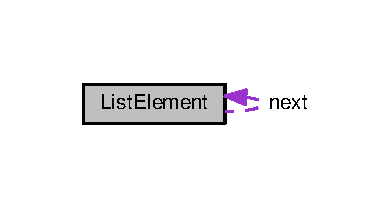
\includegraphics[width=188pt]{class_list_element__coll__graph}
\end{center}
\end{figure}
\subsection*{Public Member Functions}
\begin{DoxyCompactItemize}
\item 
{\bfseries List\+Element} (void $\ast$item\+Ptr, long long sort\+Key)\label{class_list_element_a1c8d6f93347462ddc05ad0465377ba1e}

\end{DoxyCompactItemize}
\subsection*{Public Attributes}
\begin{DoxyCompactItemize}
\item 
{\bf List\+Element} $\ast$ {\bfseries next}\label{class_list_element_aa8c417b2eb8a7b1e84dd9a2306624e61}

\item 
long long {\bfseries key}\label{class_list_element_a582785cee7d64d9397b7977e56c0185a}

\item 
void $\ast$ {\bfseries item}\label{class_list_element_ae138c41c51b6082a7b68db132f679e1e}

\end{DoxyCompactItemize}


\subsection{Detailed Description}


Definition at line 27 of file list.\+h.



The documentation for this class was generated from the following files\+:\begin{DoxyCompactItemize}
\item 
code/threads/list.\+h\item 
code/threads/list.\+cc\end{DoxyCompactItemize}

\section{Lock Class Reference}
\label{class_lock}\index{Lock@{Lock}}
\subsection*{Public Member Functions}
\begin{DoxyCompactItemize}
\item 
{\bfseries Lock} (const char $\ast$debug\+Name)\label{class_lock_afe45a309ecbd6b3346db887a76f0a9cf}

\item 
const char $\ast$ {\bfseries get\+Name} () const \label{class_lock_ad31cd7d145c782f4fefafe71277ba6cd}

\item 
void {\bfseries Acquire} ()\label{class_lock_ad4c4699fd1ab73f3927b10edc01c54db}

\item 
void {\bfseries Release} ()\label{class_lock_a5ca005b84272e56c2bf447056ee9217c}

\item 
bool {\bfseries is\+Held\+By\+Current\+Thread} () const \label{class_lock_a90db4d305ded28ee12ed08cd4c3c4d8a}

\end{DoxyCompactItemize}


\subsection{Detailed Description}


Definition at line 77 of file synch.\+h.



The documentation for this class was generated from the following files\+:\begin{DoxyCompactItemize}
\item 
code/threads/synch.\+h\item 
code/threads/synch.\+cc\end{DoxyCompactItemize}

\section{Machine Class Reference}
\label{class_machine}\index{Machine@{Machine}}


Collaboration diagram for Machine\+:\nopagebreak
\begin{figure}[H]
\begin{center}
\leavevmode
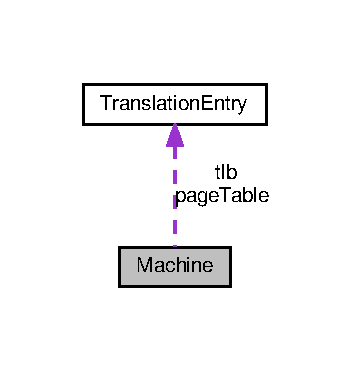
\includegraphics[width=170pt]{class_machine__coll__graph}
\end{center}
\end{figure}
\subsection*{Public Member Functions}
\begin{DoxyCompactItemize}
\item 
{\bfseries Machine} (bool debug)\label{class_machine_ad5958275a54dbc299b71ecdba7da0604}

\item 
void {\bfseries Run} ()\label{class_machine_a83444e06eb7a7c163a1b9c87a7062d43}

\item 
int {\bfseries Read\+Register} (int num)\label{class_machine_a6a8ed459cb3700c406564db72957bae3}

\item 
void {\bfseries Write\+Register} (int num, int value)\label{class_machine_ad58cc61e347395586a1cb91272dc4d61}

\item 
void {\bfseries One\+Instruction} ({\bf Instruction} $\ast$instr)\label{class_machine_af8d77f2964313173f1bada56bc596e48}

\item 
void {\bfseries Delayed\+Load} (int next\+Reg, int next\+Val)\label{class_machine_a11fda0ddf1f16d8b1a06f75d1ab5b8a1}

\item 
bool {\bfseries Read\+Mem} (int addr, int size, int $\ast$value)\label{class_machine_a01f1647867db027c04b6290b46dd988d}

\item 
bool {\bfseries Write\+Mem} (int addr, int size, int value)\label{class_machine_a1f442601e649b537a65b8b2440342227}

\item 
Exception\+Type {\bfseries Translate} (int virt\+Addr, int $\ast$phys\+Addr, int size, bool writing)\label{class_machine_a754ddcbc077cc91463398de8b0f1d077}

\item 
void {\bfseries Raise\+Exception} (Exception\+Type which, int bad\+V\+Addr)\label{class_machine_a0d6f63790c0568437b100171f61fd77f}

\item 
void {\bfseries Debugger} ()\label{class_machine_a08d36bd75e689830c73e307e1c7f7e28}

\item 
void {\bfseries Dump\+State} ()\label{class_machine_a4e4dee4ed66da41de9bbebb161efd06f}

\end{DoxyCompactItemize}
\subsection*{Public Attributes}
\begin{DoxyCompactItemize}
\item 
char $\ast$ {\bfseries main\+Memory}\label{class_machine_aa2ad571478bcc8aa88cebe50fc533ec7}

\item 
int {\bfseries registers} [Num\+Total\+Regs]\label{class_machine_a97712e3db6165648d169598fdf26b756}

\item 
{\bf Translation\+Entry} $\ast$ {\bfseries tlb}\label{class_machine_a900108b92c72cfbcab9106d99be5a315}

\item 
{\bf Translation\+Entry} $\ast$ {\bfseries page\+Table}\label{class_machine_a9e4092e3d7bab29b7d1f54ad005527ca}

\item 
unsigned int {\bfseries page\+Table\+Size}\label{class_machine_a439af96b1d906dbea5dfb538d8491418}

\end{DoxyCompactItemize}


\subsection{Detailed Description}


Definition at line 107 of file machine.\+h.



The documentation for this class was generated from the following files\+:\begin{DoxyCompactItemize}
\item 
code/machine/machine.\+h\item 
code/machine/machine.\+cc\item 
code/machine/mipssim.\+cc\item 
code/machine/translate.\+cc\end{DoxyCompactItemize}

\section{Mail Class Reference}
\label{class_mail}\index{Mail@{Mail}}


Collaboration diagram for Mail\+:\nopagebreak
\begin{figure}[H]
\begin{center}
\leavevmode
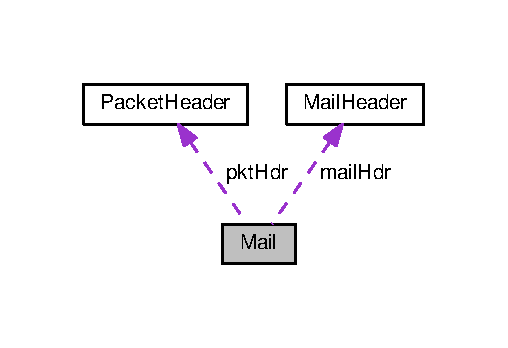
\includegraphics[width=244pt]{class_mail__coll__graph}
\end{center}
\end{figure}
\subsection*{Public Member Functions}
\begin{DoxyCompactItemize}
\item 
{\bfseries Mail} ({\bf Packet\+Header} pktH, {\bf Mail\+Header} mailH, char $\ast$msg\+Data)\label{class_mail_a25507f11e0e61e0bc84b6667650a9090}

\end{DoxyCompactItemize}
\subsection*{Public Attributes}
\begin{DoxyCompactItemize}
\item 
{\bf Packet\+Header} {\bfseries pkt\+Hdr}\label{class_mail_a7309e530849e6c8344975eaba744af5f}

\item 
{\bf Mail\+Header} {\bfseries mail\+Hdr}\label{class_mail_a1409880dfb35487ddb6d7373a4322281}

\item 
char {\bfseries data} [Max\+Mail\+Size]\label{class_mail_a6c05d7e6f61ab0c8e085690923ee7e93}

\end{DoxyCompactItemize}


\subsection{Detailed Description}


Definition at line 62 of file post.\+h.



The documentation for this class was generated from the following files\+:\begin{DoxyCompactItemize}
\item 
code/network/post.\+h\item 
code/network/post.\+cc\end{DoxyCompactItemize}

\section{Mail\+Box Class Reference}
\label{class_mail_box}\index{Mail\+Box@{Mail\+Box}}
\subsection*{Public Member Functions}
\begin{DoxyCompactItemize}
\item 
void {\bfseries Put} ({\bf Packet\+Header} pkt\+Hdr, {\bf Mail\+Header} mail\+Hdr, char $\ast$data)\label{class_mail_box_ad3c3f85a2bc7e49081e7d8b793b1ef6f}

\item 
void {\bfseries Get} ({\bf Packet\+Header} $\ast$pkt\+Hdr, {\bf Mail\+Header} $\ast$mail\+Hdr, char $\ast$data)\label{class_mail_box_a4eda4fa3299b15d8c0cf23d620676524}

\end{DoxyCompactItemize}


\subsection{Detailed Description}


Definition at line 78 of file post.\+h.



The documentation for this class was generated from the following files\+:\begin{DoxyCompactItemize}
\item 
code/network/post.\+h\item 
code/network/post.\+cc\end{DoxyCompactItemize}

\section{Mail\+Header Class Reference}
\label{class_mail_header}\index{Mail\+Header@{Mail\+Header}}
\subsection*{Public Attributes}
\begin{DoxyCompactItemize}
\item 
Mail\+Box\+Address {\bfseries to}\label{class_mail_header_ae89eec1e19689892edbeed1a98782c3a}

\item 
Mail\+Box\+Address {\bfseries from}\label{class_mail_header_aecd770168405c941b31ff1baf390df79}

\item 
unsigned {\bfseries length}\label{class_mail_header_a58dab2045076ca8bdd8bb43f21025104}

\end{DoxyCompactItemize}


\subsection{Detailed Description}


Definition at line 42 of file post.\+h.



The documentation for this class was generated from the following file\+:\begin{DoxyCompactItemize}
\item 
code/network/post.\+h\end{DoxyCompactItemize}

\section{Network Class Reference}
\label{class_network}\index{Network@{Network}}
\subsection*{Public Member Functions}
\begin{DoxyCompactItemize}
\item 
{\bfseries Network} (Network\+Address addr, double reliability, Void\+Function\+Ptr read\+Avail, Void\+Function\+Ptr write\+Done, int call\+Arg)\label{class_network_a0293c87c8c600e73383252a7c54b7c74}

\item 
void {\bfseries Send} ({\bf Packet\+Header} hdr, char $\ast$data)\label{class_network_ab68e75d65ef18f8a94a2f002c9e7f4ca}

\item 
{\bf Packet\+Header} {\bfseries Receive} (char $\ast$data)\label{class_network_a65fc6c013612cd582c099e46c1395066}

\item 
void {\bfseries Send\+Done} ()\label{class_network_ace79fd02d0d8404789162e991df951fe}

\item 
void {\bfseries Check\+Pkt\+Avail} ()\label{class_network_af33f61b6bb77606dc25805578e71abd0}

\end{DoxyCompactItemize}


\subsection{Detailed Description}


Definition at line 55 of file network.\+h.



The documentation for this class was generated from the following files\+:\begin{DoxyCompactItemize}
\item 
code/machine/network.\+h\item 
code/machine/network.\+cc\end{DoxyCompactItemize}

\section{Open\+File Class Reference}
\label{class_open_file}\index{Open\+File@{Open\+File}}
\subsection*{Public Member Functions}
\begin{DoxyCompactItemize}
\item 
{\bfseries Open\+File} (int sector)\label{class_open_file_a89136ac6b54013a413398f9496d39963}

\item 
void {\bfseries Seek} (int position)\label{class_open_file_a00f20ca65c80be4e6039a9f04cb03374}

\item 
int {\bfseries Read} (char $\ast$into, int num\+Bytes)\label{class_open_file_af87bf2b0b15fa3501dada45a1a284bf4}

\item 
int {\bfseries Write} (const char $\ast$from, int num\+Bytes)\label{class_open_file_a87c9a57b565f2503d59a1e32f68163c9}

\item 
int {\bfseries Read\+At} (char $\ast$into, int num\+Bytes, int position)\label{class_open_file_a0af8cd52ec71a2ad407039cebee2ef3d}

\item 
int {\bfseries Write\+At} (const char $\ast$from, int num\+Bytes, int position)\label{class_open_file_afdafc019e4fa166c44e8f7d4f820166f}

\item 
int {\bfseries Length} ()\label{class_open_file_a5d5618da2388829f294c3f33017fadac}

\end{DoxyCompactItemize}


\subsection{Detailed Description}


Definition at line 64 of file openfile.\+h.



The documentation for this class was generated from the following files\+:\begin{DoxyCompactItemize}
\item 
code/filesys/openfile.\+h\item 
code/filesys/openfile.\+cc\end{DoxyCompactItemize}

\section{Op\+Info Struct Reference}
\label{struct_op_info}\index{Op\+Info@{Op\+Info}}
\subsection*{Public Attributes}
\begin{DoxyCompactItemize}
\item 
int {\bfseries op\+Code}\label{struct_op_info_ae9879a2920b1ee78b2c25985eed94db9}

\item 
int {\bfseries format}\label{struct_op_info_a9b1a1704e5b5d3ccbf063c8481f31fbe}

\end{DoxyCompactItemize}


\subsection{Detailed Description}


Definition at line 112 of file mipssim.\+h.



The documentation for this struct was generated from the following file\+:\begin{DoxyCompactItemize}
\item 
code/machine/mipssim.\+h\end{DoxyCompactItemize}

\section{Op\+String Struct Reference}
\label{struct_op_string}\index{Op\+String@{Op\+String}}
\subsection*{Public Attributes}
\begin{DoxyCompactItemize}
\item 
const char $\ast$ {\bfseries string}\label{struct_op_string_a342f626cc6f66e8884c31fcf8c605bd4}

\item 
Reg\+Type {\bfseries args} [3]\label{struct_op_string_abcda212d60e80e7e6fc6ec2ca2e7ff94}

\end{DoxyCompactItemize}


\subsection{Detailed Description}


Definition at line 157 of file mipssim.\+h.



The documentation for this struct was generated from the following file\+:\begin{DoxyCompactItemize}
\item 
code/machine/mipssim.\+h\end{DoxyCompactItemize}

\section{Packet\+Header Class Reference}
\label{class_packet_header}\index{Packet\+Header@{Packet\+Header}}
\subsection*{Public Attributes}
\begin{DoxyCompactItemize}
\item 
Network\+Address {\bfseries to}\label{class_packet_header_a928d5f00dfc8c7ef789b40c7e23482a6}

\item 
Network\+Address {\bfseries from}\label{class_packet_header_ae385e650d708b1682c5705ce20dbb6c1}

\item 
unsigned {\bfseries length}\label{class_packet_header_aae6f56002b452b6dc43828fbf1a37699}

\end{DoxyCompactItemize}


\subsection{Detailed Description}


Definition at line 31 of file network.\+h.



The documentation for this class was generated from the following file\+:\begin{DoxyCompactItemize}
\item 
code/machine/network.\+h\end{DoxyCompactItemize}

\section{Pending\+Interrupt Class Reference}
\label{class_pending_interrupt}\index{Pending\+Interrupt@{Pending\+Interrupt}}
\subsection*{Public Member Functions}
\begin{DoxyCompactItemize}
\item 
{\bfseries Pending\+Interrupt} (Void\+Function\+Ptr func, int param, long long time, Int\+Type kind)\label{class_pending_interrupt_adcb5308d9a24cac163a73254e3da76cb}

\end{DoxyCompactItemize}
\subsection*{Public Attributes}
\begin{DoxyCompactItemize}
\item 
Void\+Function\+Ptr {\bfseries handler}\label{class_pending_interrupt_a4e39241c89b2e3040286333e9f83ea7d}

\item 
int {\bfseries arg}\label{class_pending_interrupt_a6484e4d50ddf69562125af75f31bda5d}

\item 
long long {\bfseries when}\label{class_pending_interrupt_a182f9d9179ea53547d19e96a2312f10a}

\item 
Int\+Type {\bfseries type}\label{class_pending_interrupt_a1ffee584e6fd0f25be17d01c4f5a5151}

\end{DoxyCompactItemize}


\subsection{Detailed Description}


Definition at line 59 of file interrupt.\+h.



The documentation for this class was generated from the following files\+:\begin{DoxyCompactItemize}
\item 
code/machine/interrupt.\+h\item 
code/machine/interrupt.\+cc\end{DoxyCompactItemize}

\section{Post\+Office Class Reference}
\label{class_post_office}\index{Post\+Office@{Post\+Office}}
\subsection*{Public Member Functions}
\begin{DoxyCompactItemize}
\item 
{\bfseries Post\+Office} (Network\+Address addr, double reliability, int n\+Boxes)\label{class_post_office_af79d08378025395d9e5fbcb62fc508cb}

\item 
void {\bfseries Send} ({\bf Packet\+Header} pkt\+Hdr, {\bf Mail\+Header} mail\+Hdr, const char $\ast$data)\label{class_post_office_a06fa263f4cd816e35c8aa78c5168f21f}

\item 
void {\bfseries Receive} (int box, {\bf Packet\+Header} $\ast$pkt\+Hdr, {\bf Mail\+Header} $\ast$mail\+Hdr, char $\ast$data)\label{class_post_office_a933ada80e0a7a5f360b80a26134b5f53}

\item 
void {\bfseries Postal\+Delivery} ()\label{class_post_office_a67ca2cc25e411b1e83580728d8fcfea8}

\item 
void {\bfseries Packet\+Sent} ()\label{class_post_office_aab32fd95c48b517b274f4e20bf16e775}

\item 
void {\bfseries Incoming\+Packet} ()\label{class_post_office_a4f1c8896b71f3ef617e106baf1d08e59}

\end{DoxyCompactItemize}


\subsection{Detailed Description}


Definition at line 102 of file post.\+h.



The documentation for this class was generated from the following files\+:\begin{DoxyCompactItemize}
\item 
code/network/post.\+h\item 
code/network/post.\+cc\end{DoxyCompactItemize}

\section{Scheduler Class Reference}
\label{class_scheduler}\index{Scheduler@{Scheduler}}
\subsection*{Public Member Functions}
\begin{DoxyCompactItemize}
\item 
void {\bfseries Ready\+To\+Run} ({\bf Thread} $\ast$thread)\label{class_scheduler_a18e89ab130a40c423da77673f12585d7}

\item 
{\bf Thread} $\ast$ {\bfseries Find\+Next\+To\+Run} ()\label{class_scheduler_a0fa7daec8d1058a8e6b5cbfbdd09555e}

\item 
void {\bfseries Run} ({\bf Thread} $\ast$next\+Thread)\label{class_scheduler_a87205b0773d3dd84752ec779c890f5e1}

\item 
void {\bfseries Print} ()\label{class_scheduler_ae82d9a7b506449c5a32d29b81e536076}

\end{DoxyCompactItemize}


\subsection{Detailed Description}


Definition at line 20 of file scheduler.\+h.



The documentation for this class was generated from the following files\+:\begin{DoxyCompactItemize}
\item 
code/threads/scheduler.\+h\item 
code/threads/scheduler.\+cc\end{DoxyCompactItemize}

\section{Semaphore Class Reference}
\label{class_semaphore}\index{Semaphore@{Semaphore}}
\subsection*{Public Member Functions}
\begin{DoxyCompactItemize}
\item 
{\bfseries Semaphore} (const char $\ast$debug\+Name, int initial\+Value)\label{class_semaphore_a671a20336d97ab712cc84aab3381d34d}

\item 
const char $\ast$ {\bfseries get\+Name} ()\label{class_semaphore_a42700933286df899977950787b46499e}

\item 
void {\bfseries P} ()\label{class_semaphore_a4fee22da0205e3c704b08beaa17e0e7a}

\item 
void {\bfseries V} ()\label{class_semaphore_a3e42125b95660ef696d0d0069b804343}

\item 
int {\bfseries E} () const \label{class_semaphore_a6dfbe972eda8b7ce2305b321aa103676}

\end{DoxyCompactItemize}


\subsection{Detailed Description}


Definition at line 39 of file synch.\+h.



The documentation for this class was generated from the following files\+:\begin{DoxyCompactItemize}
\item 
code/threads/synch.\+h\item 
code/threads/synch.\+cc\end{DoxyCompactItemize}

\section{Statistics Class Reference}
\label{class_statistics}\index{Statistics@{Statistics}}
\subsection*{Public Member Functions}
\begin{DoxyCompactItemize}
\item 
void {\bfseries Print} ()\label{class_statistics_ade67669fb1436e69a215a780b1ade63e}

\end{DoxyCompactItemize}
\subsection*{Public Attributes}
\begin{DoxyCompactItemize}
\item 
long long {\bfseries total\+Ticks}\label{class_statistics_a58b71304ed886f7b6bf4f0a098de95d6}

\item 
long long {\bfseries idle\+Ticks}\label{class_statistics_a93f73fe07546a65cccc257fe36d22f7d}

\item 
long long {\bfseries system\+Ticks}\label{class_statistics_a1b863346650d845fd66c2a82edc821b3}

\item 
long long {\bfseries user\+Ticks}\label{class_statistics_abf5ff8cdf5bca15c2a48eb48e11a15a8}

\item 
int {\bfseries num\+Disk\+Reads}\label{class_statistics_a50d57d5c9a5a6b07aa22ad8362259f9e}

\item 
int {\bfseries num\+Disk\+Writes}\label{class_statistics_a5c1854b002d360cdb1dff4438fa6e30f}

\item 
int {\bfseries num\+Console\+Chars\+Read}\label{class_statistics_ab5ea51542ab83433169760d71452a305}

\item 
int {\bfseries num\+Console\+Chars\+Written}\label{class_statistics_a67aa7a06b0933ad257608174f3123e6e}

\item 
int {\bfseries num\+Page\+Faults}\label{class_statistics_a0178d49a84e5dcc4a7672dc973e8f586}

\item 
int {\bfseries num\+Packets\+Sent}\label{class_statistics_a7ccdb4de272140b26cf54efc5dec5cf0}

\item 
int {\bfseries num\+Packets\+Recvd}\label{class_statistics_a0907df803623b828b76be1efba2d3c56}

\end{DoxyCompactItemize}


\subsection{Detailed Description}


Definition at line 22 of file stats.\+h.



The documentation for this class was generated from the following files\+:\begin{DoxyCompactItemize}
\item 
code/machine/stats.\+h\item 
code/machine/stats.\+cc\end{DoxyCompactItemize}

\section{Synch\+Console Class Reference}
\label{class_synch_console}\index{Synch\+Console@{Synch\+Console}}


Inheritance diagram for Synch\+Console\+:\nopagebreak
\begin{figure}[H]
\begin{center}
\leavevmode
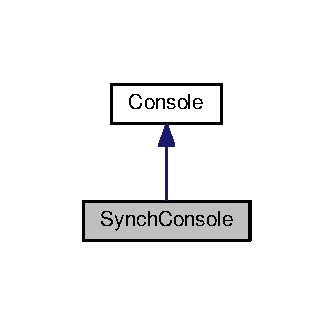
\includegraphics[width=160pt]{class_synch_console__inherit__graph}
\end{center}
\end{figure}


Collaboration diagram for Synch\+Console\+:\nopagebreak
\begin{figure}[H]
\begin{center}
\leavevmode
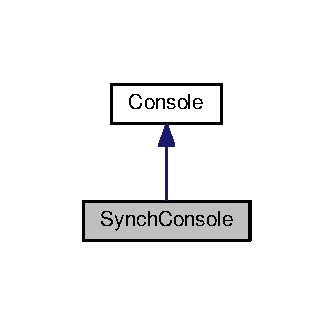
\includegraphics[width=160pt]{class_synch_console__coll__graph}
\end{center}
\end{figure}
\subsection*{Public Member Functions}
\begin{DoxyCompactItemize}
\item 
{\bfseries Synch\+Console} (char $\ast$read\+File, char $\ast$write\+File)\label{class_synch_console_a888915fb5c11051308853603ccf0e436}

\item 
void {\bfseries Put\+Char} (const char ch)\label{class_synch_console_a604aabb23deed2795dccd343d63c5692}

\item 
int {\bfseries Get\+Char} ()\label{class_synch_console_a58ca9990bb4eea2acb7f42e340b10d26}

\item 
void {\bfseries Put\+String} (const char $\ast$s)\label{class_synch_console_a418e6285c64156cee661cb6fbffae5e7}

\item 
void {\bfseries Get\+String} (char $\ast$s, int n)\label{class_synch_console_a2003d238e6fb4fa6a3a2b8ff31bedd7e}

\item 
void {\bfseries handler\+Read\+Avail} ()\label{class_synch_console_ab4f1b48fbf66efb13e7b8ff7fe8c930a}

\item 
void {\bfseries handler\+Write\+Done} ()\label{class_synch_console_a7537f191fbc6a4e5e78478f4d985c10c}

\end{DoxyCompactItemize}
\subsection*{Static Public Member Functions}
\begin{DoxyCompactItemize}
\item 
static void {\bfseries handler\+Read\+Avail} (int)\label{class_synch_console_ab15b6af88078b3cc8f88f1f19cb7e66d}

\item 
static void {\bfseries handler\+Write\+Done} (int)\label{class_synch_console_ab3eb4e79b68ae8f4acefe51789819add}

\end{DoxyCompactItemize}


\subsection{Detailed Description}


Definition at line 10 of file synchconsole.\+h.



The documentation for this class was generated from the following files\+:\begin{DoxyCompactItemize}
\item 
code/userprog/synchconsole.\+h\item 
code/userprog/synchconsole.\+cc\end{DoxyCompactItemize}

\section{Synch\+Disk Class Reference}
\label{class_synch_disk}\index{Synch\+Disk@{Synch\+Disk}}
\subsection*{Public Member Functions}
\begin{DoxyCompactItemize}
\item 
{\bfseries Synch\+Disk} (const char $\ast$name)\label{class_synch_disk_aa6cc1815e0aca2d6fe11d426942e6538}

\item 
void {\bfseries Read\+Sector} (int sector\+Number, char $\ast$data)\label{class_synch_disk_a7d8195bd5d464e4771946eb03c61e8c8}

\item 
void {\bfseries Write\+Sector} (int sector\+Number, char $\ast$data)\label{class_synch_disk_aadb7e2ce6cf32727e493c63c5ea1018b}

\item 
void {\bfseries Request\+Done} ()\label{class_synch_disk_a973a65b7b7b92f5fabf18da8b8bae402}

\end{DoxyCompactItemize}


\subsection{Detailed Description}


Definition at line 27 of file synchdisk.\+h.



The documentation for this class was generated from the following files\+:\begin{DoxyCompactItemize}
\item 
code/filesys/synchdisk.\+h\item 
code/filesys/synchdisk.\+cc\end{DoxyCompactItemize}

\section{Synch\+List Class Reference}
\label{class_synch_list}\index{Synch\+List@{Synch\+List}}
\subsection*{Public Member Functions}
\begin{DoxyCompactItemize}
\item 
void {\bfseries Append} (void $\ast$item)\label{class_synch_list_a8cd56b067f02d53025d8078f748e6b75}

\item 
void $\ast$ {\bfseries Remove} ()\label{class_synch_list_afe8d909e1ab9dce01ddd7d24716be56f}

\item 
void {\bfseries Mapcar} (Void\+Function\+Ptr func)\label{class_synch_list_ac9faf4621078baddee6890b0e184fc2d}

\end{DoxyCompactItemize}


\subsection{Detailed Description}


Definition at line 24 of file synchlist.\+h.



The documentation for this class was generated from the following files\+:\begin{DoxyCompactItemize}
\item 
code/threads/synchlist.\+h\item 
code/threads/synchlist.\+cc\end{DoxyCompactItemize}

\section{Thread Class Reference}
\label{class_thread}\index{Thread@{Thread}}
\subsection*{Public Member Functions}
\begin{DoxyCompactItemize}
\item 
{\bfseries Thread} (const char $\ast$debug\+Name)\label{class_thread_aeef00ecb5eda30734cff97a0ac492bdd}

\item 
void {\bfseries Fork} (Void\+Function\+Ptr func, int arg)\label{class_thread_a7631955bc5e11232bb682baa467baf5f}

\item 
void {\bfseries Yield} ()\label{class_thread_adbc2bfb172d2eff4b46882aade9eeb8a}

\item 
void {\bfseries Sleep} ()\label{class_thread_a187a4c1e62087511b69068220840244a}

\item 
void {\bfseries Finish} ()\label{class_thread_a1e43c788c40e9783311c970bcea7239b}

\item 
void {\bfseries Check\+Overflow} ()\label{class_thread_afa6657ff14b9c6866eadd85ea32c9147}

\item 
void {\bfseries set\+Status} (Thread\+Status st)\label{class_thread_a39061ce2692542188f82f909d005b1c3}

\item 
const char $\ast$ {\bfseries get\+Name} ()\label{class_thread_aed303e0688ec792e41fb9b7429a3d948}

\item 
void {\bfseries Print} ()\label{class_thread_ad707af00a9ce1a1d324804e7c73dc4ab}

\end{DoxyCompactItemize}


\subsection{Detailed Description}


Definition at line 77 of file thread.\+h.



The documentation for this class was generated from the following files\+:\begin{DoxyCompactItemize}
\item 
code/threads/thread.\+h\item 
code/threads/thread.\+cc\end{DoxyCompactItemize}

\section{Timer Class Reference}
\label{class_timer}\index{Timer@{Timer}}
\subsection*{Public Member Functions}
\begin{DoxyCompactItemize}
\item 
{\bfseries Timer} (Void\+Function\+Ptr timer\+Handler, int call\+Arg, bool do\+Random)\label{class_timer_ad6f578a6b75f1073e7c6919cf8a507ee}

\item 
void {\bfseries Timer\+Expired} ()\label{class_timer_ad0198c93d207f2f303b3c5ff5cfd8ef4}

\item 
int {\bfseries Time\+Of\+Next\+Interrupt} ()\label{class_timer_a2846bc4b6ef4ad61e3de987aee4d85ab}

\end{DoxyCompactItemize}


\subsection{Detailed Description}


Definition at line 27 of file timer.\+h.



The documentation for this class was generated from the following files\+:\begin{DoxyCompactItemize}
\item 
code/machine/timer.\+h\item 
code/machine/timer.\+cc\end{DoxyCompactItemize}

\section{Translation\+Entry Class Reference}
\label{class_translation_entry}\index{Translation\+Entry@{Translation\+Entry}}
\subsection*{Public Attributes}
\begin{DoxyCompactItemize}
\item 
unsigned int {\bfseries virtual\+Page}\label{class_translation_entry_af7d48c86a1188e1e78f00d3eaa1b21ad}

\item 
unsigned int {\bfseries physical\+Page}\label{class_translation_entry_ada1901a6079061755592c3b5d6a4098c}

\item 
bool {\bfseries valid}\label{class_translation_entry_a655ccdb71f2e1c8bc43d751b5c375cd2}

\item 
bool {\bfseries read\+Only}\label{class_translation_entry_a99d5c440c0d011213a39edf4d0844a7d}

\item 
bool {\bfseries use}\label{class_translation_entry_acd4ec2f9980de42c849562c211a3813a}

\item 
bool {\bfseries dirty}\label{class_translation_entry_a4a198eb7773a247967dcf4e377d3717f}

\end{DoxyCompactItemize}


\subsection{Detailed Description}


Definition at line 30 of file translate.\+h.



The documentation for this class was generated from the following file\+:\begin{DoxyCompactItemize}
\item 
code/machine/translate.\+h\end{DoxyCompactItemize}

%--- End generated contents ---

% Index
\backmatter
\newpage
\phantomsection
\clearemptydoublepage
\addcontentsline{toc}{chapter}{Index}
\printindex

\end{document}
